\documentclass[conference]{IEEEtran}
\usepackage[T1]{fontenc}
\usepackage{amsmath,amssymb,graphicx,booktabs,array,url}
\usepackage[hidelinks]{hyperref}
\graphicspath{{figures/}}
\begin{document}
\title{NEERWATCH: Satellite-Based Chlorophyll-a Estimation and Temporal Water Quality Monitoring of Karnataka Reservoirs Using Sentinel-2 Imagery}
\author{\IEEEauthorblockN{[Author Name(s)]}\IEEEauthorblockA{[Department]\\{[Institution]}\\{[City, Country]}\\{[Email address(es)]}}}
\maketitle
\begin{abstract}
NEERWATCH implements satellite-derived chlorophyll-a screening and dated temporal comparison for Karnataka reservoirs. This paper documents the operational implementation and its persisted observation snapshot of 22 October 2026. Sentinel-2 Level-2A imagery is retrieved through the Microsoft Planetary Computer, aligned to a common 60 m grid, and screened using reservoir polygons, the Scene Classification Layer, buffered shoreline and cloud masks, and reflectance checks. A Gilerson-based two-band empirical expression is applied pixel-wise to red and red-edge reflectances; the median of retained pixels represents each reservoir observation. Compatible observations support absolute and percentage change calculations and EPA-based trophic screening categories. Python processing, file-based provenance storage, FastAPI services, and a React/Leaflet interface provide images, chlorophyll maps, comparisons, and PDF reports. The published inventory contains 46 reservoirs with two compatible observations each. Latest estimates span 16.18--67.65 micrograms per litre; 42 fall in the eutrophic and four in the hypereutrophic screening category. These values are experimental estimates rather than field measurements. The implementation has no independent Karnataka chlorophyll validation, and software verification does not establish retrieval accuracy. No trained machine-learning model or future concentration forecast is used in the documented monitoring path.
\end{abstract}
\begin{IEEEkeywords}
chlorophyll-a, Sentinel-2, Karnataka reservoirs, empirical estimation, temporal monitoring, geospatial web system
\end{IEEEkeywords}
\section{Introduction}
Reservoir monitoring benefits from observations that preserve both spatial coverage and acquisition time. Satellite imagery can help prioritize follow-up sampling, but translating reflectance into a water-quality concentration introduces assumptions about atmosphere, water optics, spatial mixing, and calibration. A useful operational interface must therefore expose provenance and distinguish an estimate from an independently validated measurement.

NEERWATCH addresses this engineering problem through a traceable Sentinel-2 workflow for Karnataka reservoirs. The contribution described here is an implemented acquisition-to-dashboard system: quality-screened imagery, an explicit empirical estimator, persistent spectral evidence, compatible-date comparison, and linked visualization and reporting. The work is an implementation study, not an accuracy assessment or a newly trained retrieval model. All numerical results refer to the saved project snapshot inspected on 22 October 2026.

\section{Literature Review}
\subsection{Red and Red-Edge Empirical Retrieval}
Gilerson et al.\ \cite{gilerson2010} investigate red and near-infrared algorithms for chlorophyll-a estimation in coastal and inland waters. Their work provides the scientific basis for the two-band expression adopted by this implementation. NEERWATCH retains fixed published coefficients; it does not estimate regression coefficients from Karnataka samples. Applying an aquatic-reflectance formulation to provider land-oriented bottom-of-atmosphere (BOA) reflectance is a material adaptation, and requires an explicit qualification rather than a claim of transferred accuracy.

\subsection{Published Regression-Based Related Work}
Assaf et al.\ \cite{assaf2025} integrate Sentinel-2 reflectance and in-situ chlorophyll observations and compare six regression approaches: artificial neural networks, CatBoost, random forest, ridge regression, support vector regression, and extreme gradient boosting. Their study also examines feature importance. This is relevant related work because it demonstrates a supervised, paired-data approach to chlorophyll retrieval. Those models and their reported performance are not NEERWATCH results. The current system implements an empirical expression without a locally trained regressor; the two studies have different evidential bases.

\section{Existing Research and Base Paper}
The implemented mathematical base is Gilerson et al.\ \cite{gilerson2010}; Assaf et al.\ \cite{assaf2025} provide a separate regression-based comparison in the literature. The source tree also contains a vendored WaterQual index routine\cite{waterqual}, used to compute a diagnostic normalized difference chlorophyll index. That index is not substituted for concentration. The concentration implementation explicitly evaluates the power-law expression described in Section~\ref{sec:method}. Historical training-related files elsewhere in the repository are outside the active monitoring path and provide no accuracy evidence for this paper.

\section{Problem Statement and Objectives}
The practical problem is to transform irregular usable satellite acquisitions into reservoir-specific, auditable screening observations. Different native band resolutions, cloud contamination, shoreline mixing, partial tile footprints, and mismatched dates can otherwise produce misleading concentrations or change values.

The implemented objectives are to (1) retrieve and align real Sentinel-2 spectral data within verified reservoir polygons; (2) reject unsuitable acquisitions without manufacturing results; (3) compute and preserve pixel estimates and reservoir medians; (4) compare compatible observations with explicit dates; and (5) present results, source imagery, categories, and reports through a usable geospatial interface. These objectives do not include toxicity detection or future concentration prediction.

\section{Study Area: Karnataka Reservoirs}
The published registry contains 46 Karnataka reservoirs, including KRS, Bhadra, Tungabhadra, Supa, Vani Vilasa Sagara, Kabini, Harangi, Hemavathi, Almatti, Linganamakki, Basava Sagara, and Malaprabha. Table~\ref{tab:all} lists the complete operational inventory. Reservoir identities and location checks use the project registry and associated official-record evidence, including the Central Water Commission register\cite{cwc}; water polygons retain OpenStreetMap provenance and licensing\cite{osm}. Figure~\ref{fig:study} plots the actual stored polygons and their centroids. It is a distribution plot, not an authoritative administrative boundary map.

Operational membership is narrower than a list of candidate names: each published reservoir must have a valid water polygon, location/provenance metadata, two compatible dated concentration observations, and persisted spectral and display assets. Additional internal candidates are not included in the count.
\begin{figure}[t]
\centering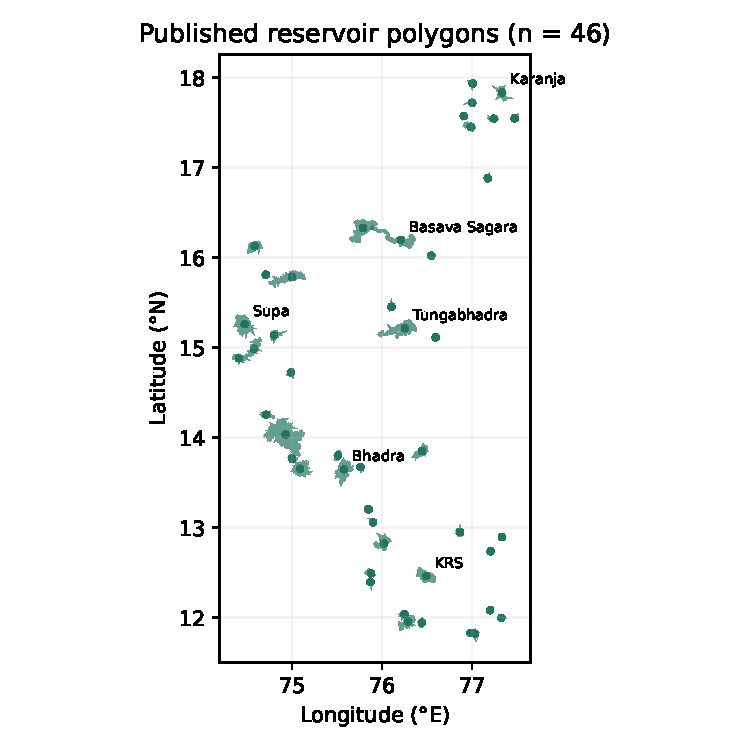
\includegraphics[width=\columnwidth]{reservoir-distribution.pdf}
\caption{Actual published reservoir geometries and centroids from the project registry. Polygons: \copyright\ OpenStreetMap contributors, ODbL 1.0. Selected names are annotated for orientation; no external basemap is implied.}\label{fig:study}
\end{figure}

\section{Data Sources}
Sentinel-2 Level-2A imagery supplies provider-corrected BOA reflectance and the Scene Classification Layer (SCL)\cite{esa}. The active acquisition path queries the Microsoft Planetary Computer STAC collection \texttt{sentinel-2-l2a}, and accesses signed cloud-optimized raster assets\cite{pc}. B04 (red) and B05 (red-edge) feed the concentration ratio. B02, B03, B08, and B11 additionally support multiband quality checks and stored diagnostics; B04/B03/B02 provide true colour.

Each saved manifest identifies the acquisition timestamp, source item, spectral assets, scale/offset, coordinate reference system, processing method, quality statistics, polygon source, and generated files. Composite observations retain their constituent scene identifiers and times. The concentration results in this paper come from those persisted Sentinel-2 assets; no Sentinel-3 concentration or field-label archive is substituted into them.

\section{Current System Architecture}
Figure~\ref{fig:arch} shows the implemented data flow. Acquisition and geometric preparation feed pixel estimation. Persisted observation files support the backend's classification and compatible-date comparison. FastAPI serves the React application and data routes; Leaflet displays the reservoir polygons. ReportLab generates reservoir PDF reports on the backend.

The storage layer consists of JSON manifests and job state, compressed NumPy spectral arrays and masks, PNG products, and GeoTIFF concentration rasters. There is no database dependency in this active path. The dashboard reads cached observations and supports manual processing requests with status polling. This does not constitute a continuously scheduled acquisition service.
\begin{figure*}[t]
\centering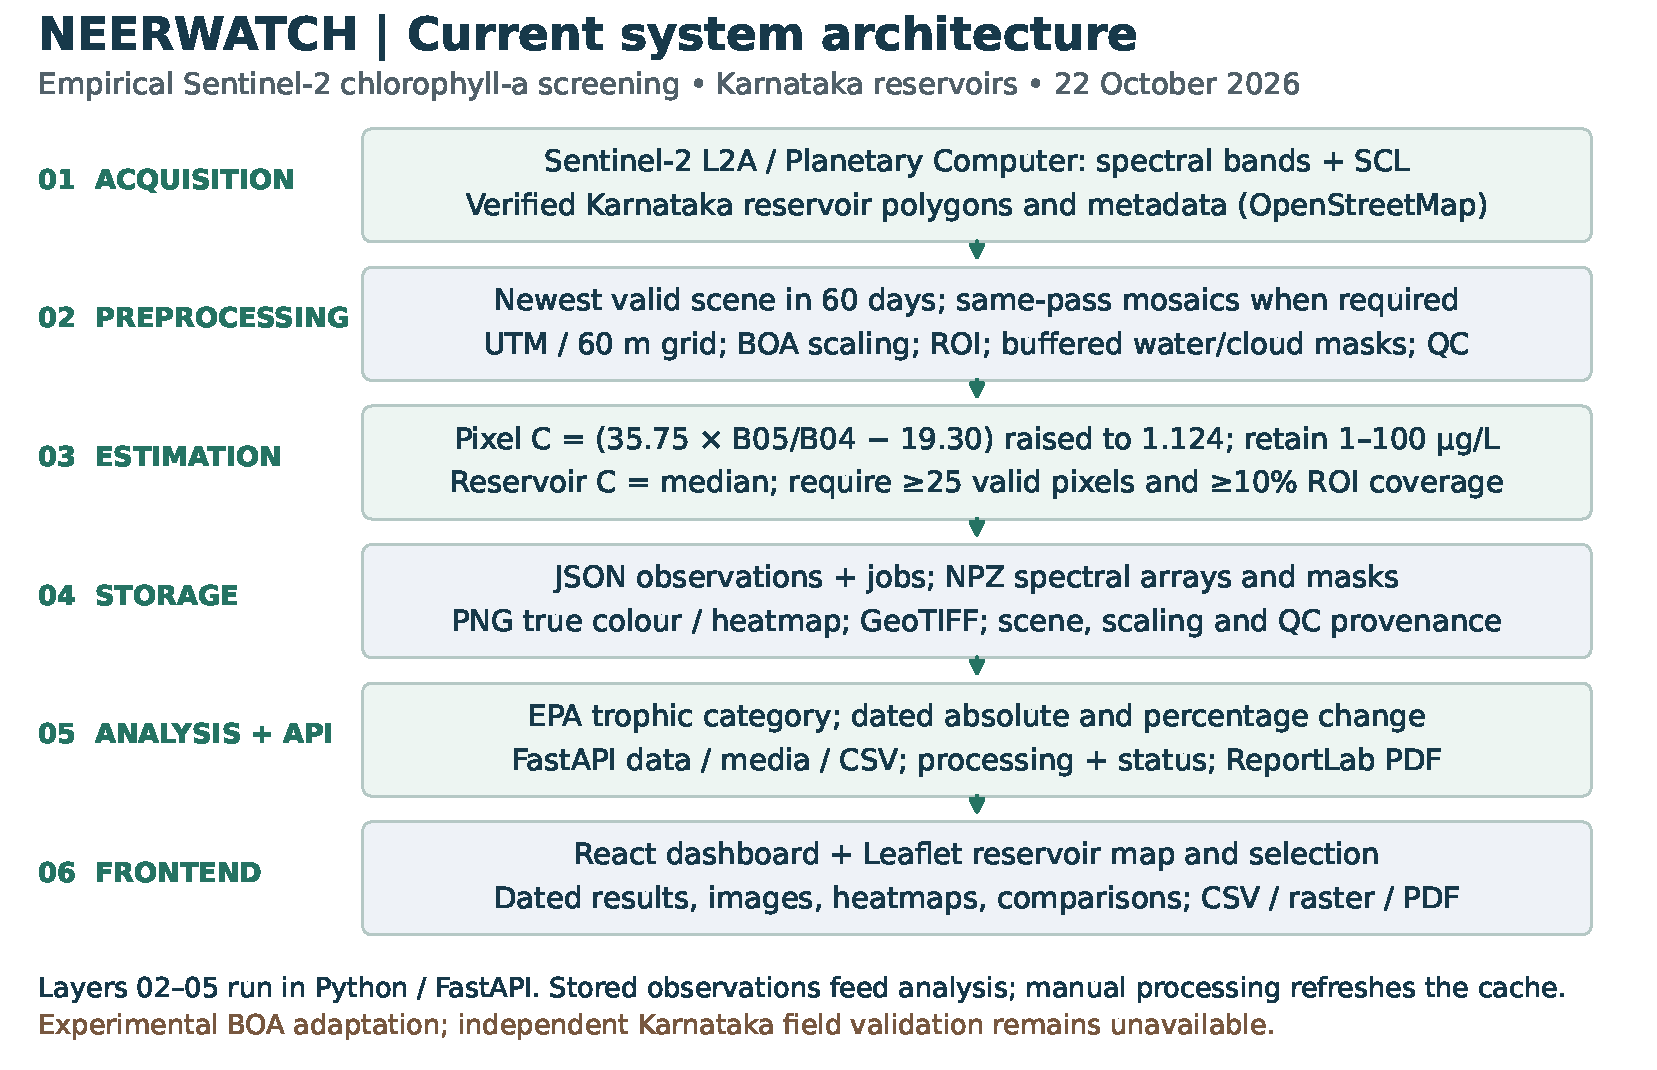
\includegraphics[width=\textwidth]{NEERWATCH_Current_Architecture.pdf}
\caption{Current empirical monitoring architecture, verified against processing, service, and interface code. The file cache supplies the API analysis layer; processing requests refresh stored observations. PDF generation executes in the Python backend.}\label{fig:arch}
\end{figure*}

\section{Methodology}\label{sec:method}
\subsection{Acquisition Selection and Same-Pass Mosaics}
A paginated STAC query searches a 60-day lookback window and orders candidate observations newest first. The processor selects the newest observation that passes all gates; a more recent rejected scene does not become a concentration result. A candidate footprint must cover at least 95\% of the reservoir polygon.

Where a single tile is insufficient, the mosaic implementation groups tiles by calendar date, platform, relative orbit, and processing baseline, with a maximum timestamp separation of 300 seconds. The union footprint and resulting mosaic data footprint must meet the 95\% requirement. A deterministic SCL-based ownership array assigns overlapping pixels to one tile across all bands. Different-day imagery is not merged. The snapshot includes same-pass composites for Basava Sagara and Malaprabha; a composite identifier must not be mistaken for a single original Sentinel scene.

\subsection{Spatial Alignment and ROI Extraction}
GeoJSON polygons in geographic coordinates are transformed to the northern UTM zone selected from the reservoir centroid. A common 60 m grid is created over the projected bounds, and raster assets are read through a nearest-neighbour warped virtual raster. B04 is natively 10 m and B05 natively 20 m in the saved metadata; the 60 m analysis grid is an implementation choice, not the native sensor resolution. A rasterized polygon mask defines the region of interest (ROI). The grid is limited to 1.5 million cells to bound processing demand.

\subsection{Reflectance Processing}
For each asset, reflectance is computed as
\begin{equation}
\rho_b=s_b\,DN_b+o_b,\label{eq:rho}
\end{equation}
where asset metadata supplies scale $s_b$ and offset $o_b$ when available. The fallback uses $s_b=10^{-4}$ and $o_b=-0.1$ for processing baseline at least 4, otherwise zero offset. Raw zero values are treated as missing. Stored per-band metadata records the actual conversion, including separate source metadata for mosaics. Additive offsets are applied before forming ratios; they do not cancel as a common multiplicative scale would.

\subsection{Cloud, Shadow, Land and Water Screening}
The candidate mask is the polygon intersected with SCL class 6 (water), eroded by one analysis pixel. Classes 3, 8, 9, and 10 (shadow/cloud/cirrus) are dilated by one pixel and excluded. At 60 m this supplies 60 m shoreline and cloud buffers. Land and other non-water SCL classes are excluded by the water requirement. All six spectral bands must be finite and satisfy $0<\rho_b\leq1$. These gates require at least 25 retained pixels and at least 10\% of polygon pixels. The denominator is the rasterized reservoir polygon, not merely the initially classified water area.

These are project screening rules, not a demonstrated uncertainty bound. Accepted observations may still represent only part of a reservoir; differing spatial support remains a limitation for temporal interpretation.

\subsection{Gilerson Chlorophyll-a Estimation}
For valid red and red-edge reflectances the exact implemented expression is
\begin{equation}
C_i=\left(35.75\frac{\rho_{B05,i}}{\rho_{B04,i}}-19.30\right)^{1.124},\label{eq:chl}
\end{equation}
with $C_i$ reported in $\mu$g/L. Both reflectances and the power-law base must be positive. Non-finite values and estimates outside $1\leq C_i\leq100$ are rejected, not clipped to a boundary value. This range is a conservative project acceptance rule, not a claimed published calibration interval.

The use of Sentinel-2 B05 near 705 nm and Sen2Cor BOA in an aquatic-reflectance formulation is experimental. Water-specific atmospheric correction, including aquatic DSF and adjacency correction, is not performed. Equation~\eqref{eq:chl} is therefore described throughout as a screening adaptation of Gilerson et al.\ \cite{gilerson2010}, not a locally calibrated concentration model.

\subsection{Aggregation and Quality Control}
The reservoir estimate is the median of retained pixel estimates:
\begin{equation}
\widehat C_r(t)=\operatorname{median}_{i\in V_{r,t}} C_i.
\end{equation}
The count and 10\% coverage gates are applied again after algorithm filtering. The processor stores the exact validity mask, spectral arrays, concentration array, median, and quality metadata. Unusable acquisitions retain rejection reasons and the processor tries earlier candidates. If no acceptable concentration is found, it reports a specific failure rather than assigning a numerical placeholder.

\subsection{EPA-Based Trophic Classification}
The implementation uses the EPA National Lakes Assessment concentration bands\cite{epa}: oligotrophic $C\leq2$, mesotrophic $2<C\leq7$, eutrophic $7<C\leq30$, and hypereutrophic $C>30$, in $\mu$g/L. Missing, negative, or non-finite concentrations receive no category. Applying these U.S. lake concentration bands to an experimental satellite estimate yields an indicative trophic screening category, not a Karnataka regulatory determination, toxin concentration, cyanobacterial dominance assessment, or drinking-water safety decision.

\subsection{Dated Temporal Comparison}
The backend selects an earlier observation from a different calendar date with matching method, atmospheric correction, resolution, masks, minimum sample/coverage settings, screening range, and aggregation. For a positive earlier concentration,
\begin{align}
\Delta C&=\widehat C_r(t_2)-\widehat C_r(t_1),\\
\Delta C_{\%}&=100\frac{\widehat C_r(t_2)-\widehat C_r(t_1)}{\widehat C_r(t_1)}.
\end{align}
The interface displays both dates; the sign determines increasing, decreasing, or unchanged. The interval is not constrained to seven days. These quantities describe two observations and are neither a forecast nor a bloom probability.

\section{System Implementation}
\subsection{Python Processing and Persistent Evidence}
NumPy evaluates the expression and aggregation; Rasterio handles raster reprojection and GeoTIFF output; Shapely handles polygon geometry; SciPy performs mask morphology. Matplotlib and Pillow generate heatmaps and true-colour products. The concentration GeoTIFF preserves its coordinate reference system and affine transform. The PNG heatmap contains a colour bar and is not claimed to be a georeferenced Leaflet raster overlay.

The processing service persists queued/running/complete/failed job state and maintains a two-worker execution pool. It records scene attempts and explicit error reasons. Persisted state supports reloads and interrupted-job detection after backend restart. Cached scene reuse avoids unnecessary repeat calculations when compatible products already exist.

\subsection{FastAPI Services}
The principal routes list and describe reservoirs, serve boundaries and scene-pinned media, export comparison CSV, initiate Sentinel-2 processing, poll job status, and return a reservoir PDF. Media selection can specify a scene identifier, keeping images tied to the displayed historical acquisition. The public inventory gate checks provenance, valid geometry, compatible observation pairs, valid units, and required persisted products before publishing a reservoir.

\subsection{React, Leaflet and Reporting}
The React interface synchronizes reservoir selection with Leaflet boundary highlighting and map extent. It displays acquisition dates, medians, category and temporal change, true-colour imagery, chlorophyll maps, and source/download links. The comparison table supports reservoir and region details, both concentrations and dates, signed changes, categories, previews, and sorting. Backend ReportLab reports summarize the selected reservoir with dated results, images, history and limitations. Figure~\ref{fig:products} reproduces actual saved satellite products; it is not a fabricated interface screenshot.
\begin{figure*}[t]
\centering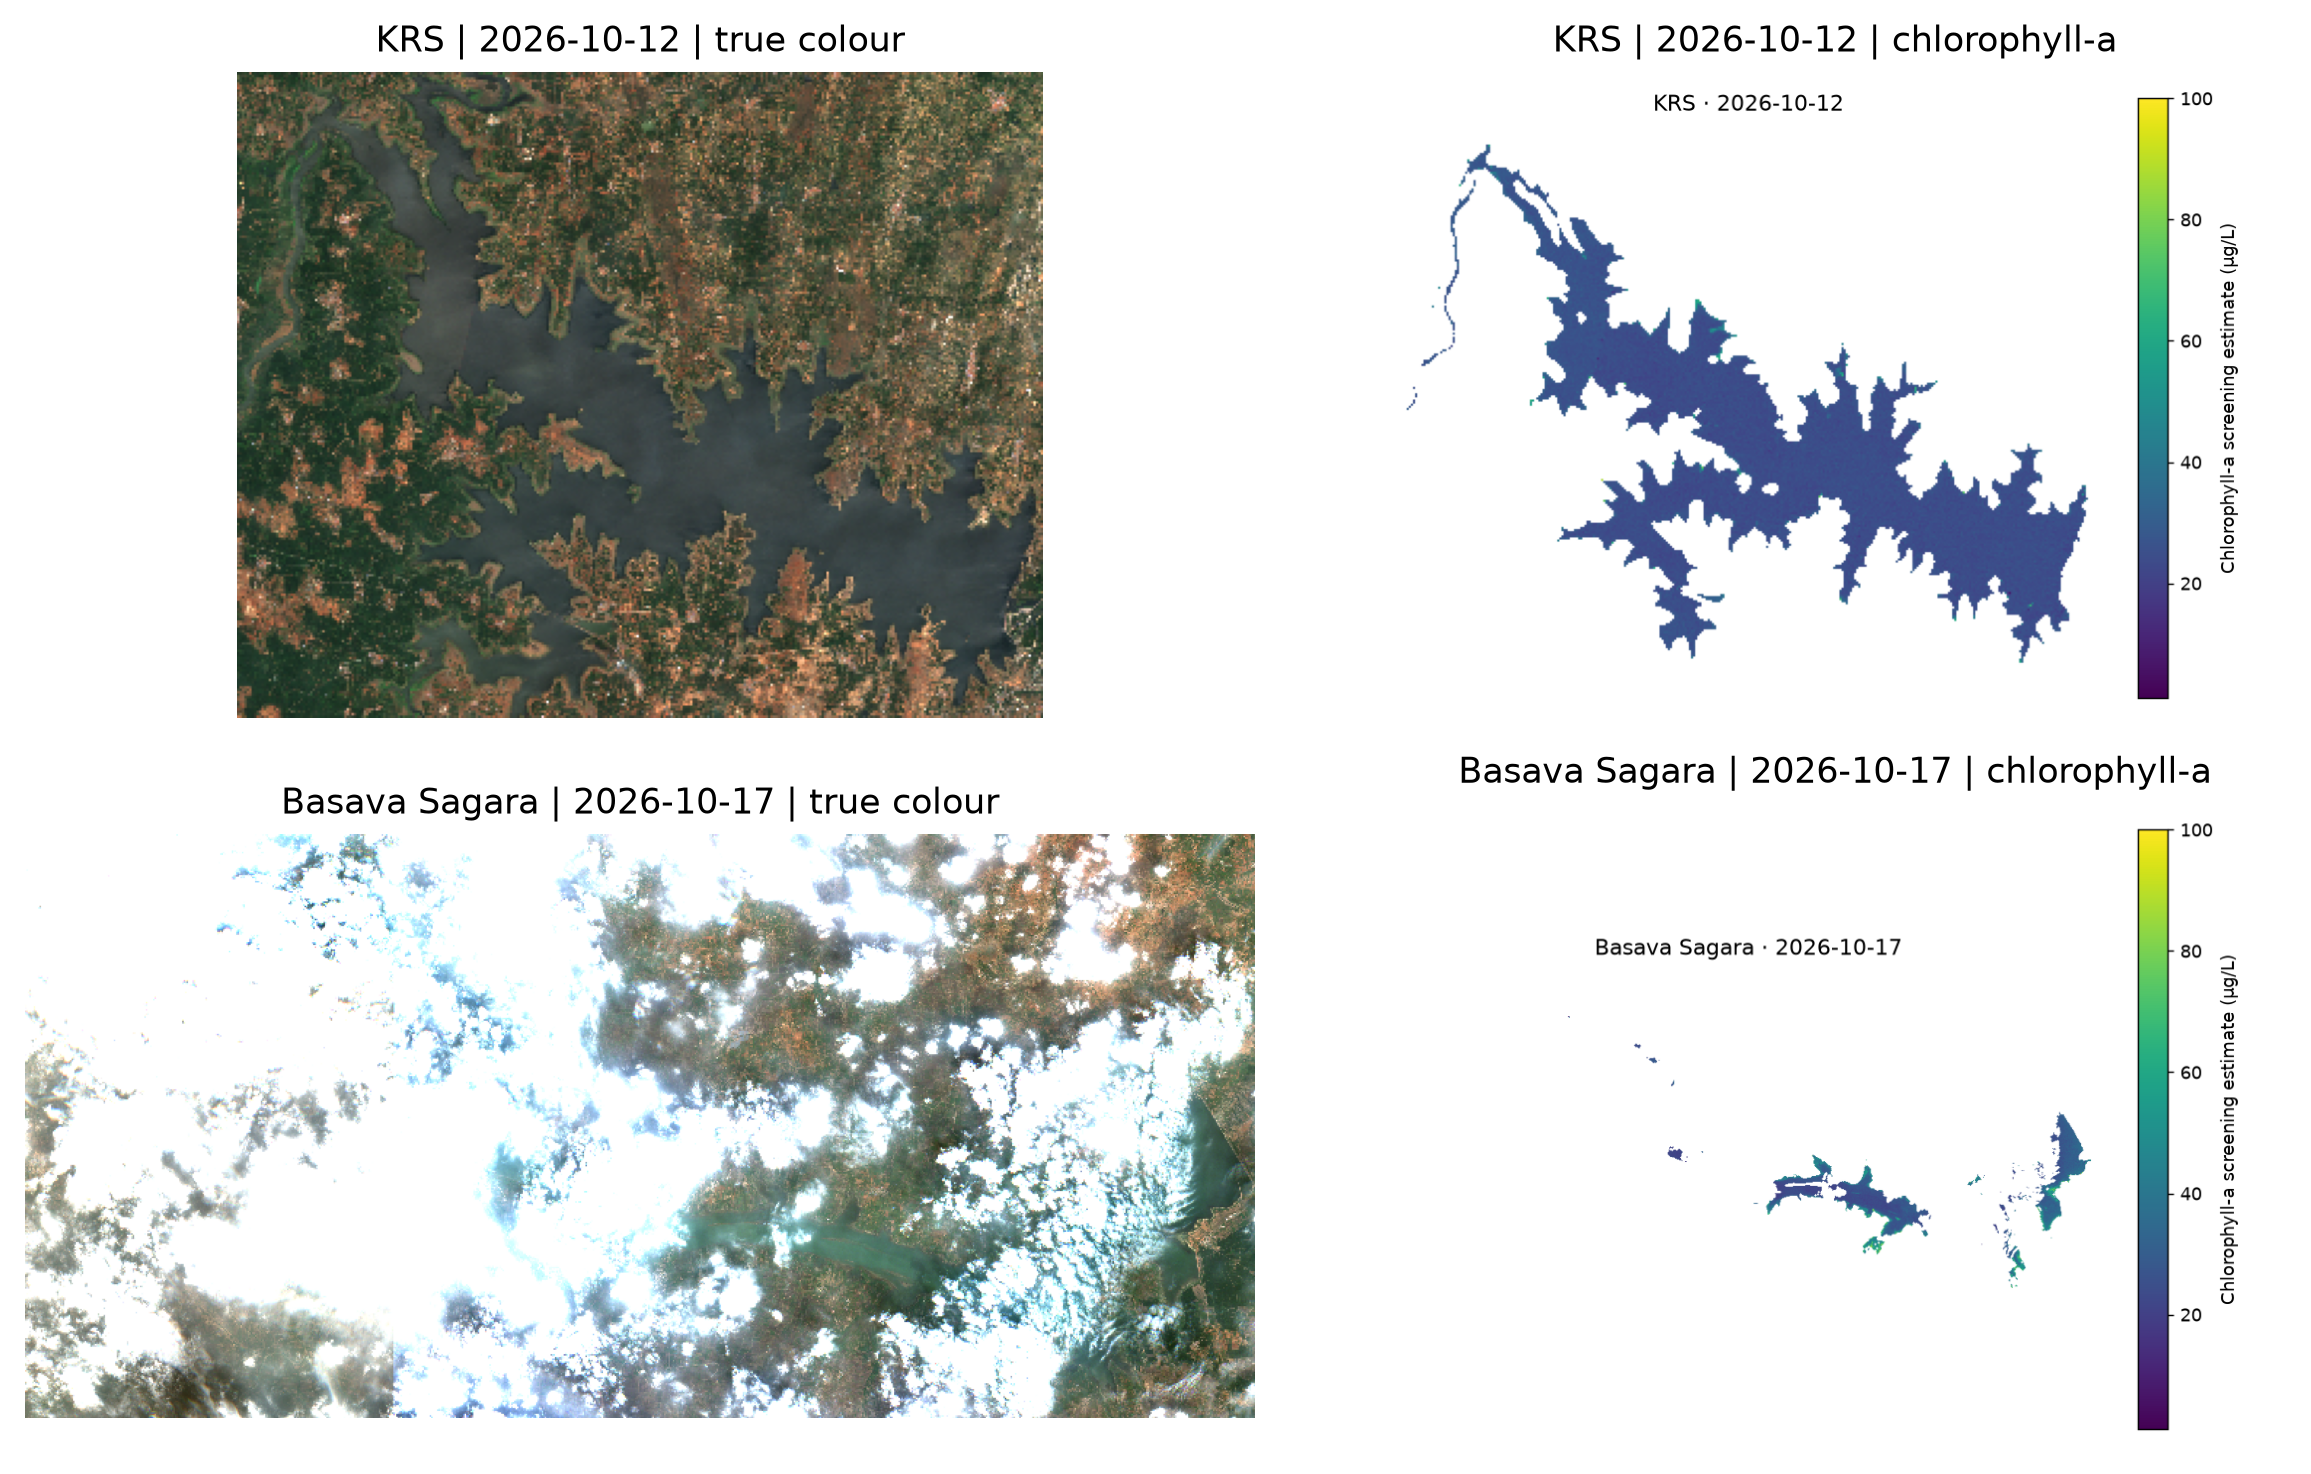
\includegraphics[width=.96\textwidth]{satellite-products.png}
\caption{Real cached products: KRS (12 October 2026, single scene) and Basava Sagara (17 October 2026, same-pass mosaic). Left: true-colour display; right: stored chlorophyll screening heatmap. Colours are estimates from the retained spectral pixels, not field observations; the fixed map scale is 1--100 $\mu$g/L. Source: Copernicus Sentinel-2 L2A through Microsoft Planetary Computer.}\label{fig:products}
\end{figure*}

\section{Results and Discussion}
\subsection{Snapshot and Numerical Reproduction}
The inspected registry contains 46 published reservoirs, each with two compatible observations: 92 reservoir-date records. Acquisition dates across these pairs span 9 September--20 October 2026. These are dates of imagery, not the document preparation date. The latest acceptable observation is not necessarily the newest satellite acquisition because cloud, water-pixel and footprint requirements reject candidates.

An independent read-only audit recomputed Equation~\eqref{eq:chl} from the saved B04/B05 arrays for all 92 records, applied the saved validity masks, and checked pixel estimates, valid-pixel counts, and reservoir medians against stored products. Reported medians agreed within $10^{-5}$ $\mu$g/L numerical tolerance. This checks implementation consistency; the cached spectral inputs themselves are not independent ground truth.

Latest reservoir estimates range from 16.18 to 67.65 $\mu$g/L. The resulting categories are 42 eutrophic and four hypereutrophic; none are oligotrophic or mesotrophic. Twenty reservoirs show a positive two-date change and 26 a negative change. Latest algorithm-valid coverage ranges from 11.60\% to 81.91\% of polygon pixels. These percentages qualify the spatial support of the medians and are not accuracy percentages.

\subsection{Representative Temporal Outcomes}
KRS decreases from 25.15 $\mu$g/L on 9 October to 24.72 on 12 October ($-1.71$\%). Bhadra decreases from 25.35 to 23.97 over those dates ($-5.46$\%). Tungabhadra increases from 27.34 on 12 October to 42.19 on 17 October ($+54.33$\%), crossing the 30 $\mu$g/L screening boundary. Supa increases from 22.68 on 10 October to 25.32 on 20 October ($+11.62$\%). These examples demonstrate why concentration category and direction of change must be shown together. A falling concentration can remain in an elevated category.

The complete results appear in Table~\ref{tab:all}. Values are rounded only for presentation; calculations use stored floating-point observations. A large percentage change over one pair does not prove a biological bloom event: clouds, residual atmospheric effects and spatially differing retained pixels can influence both medians.

\subsection{Operational Verification Versus Scientific Validation}
Existing project verification records report 60 passing backend tests and a successful frontend production build. The saved interface-state audit covers 92 reservoir workspace loads over two sessions, including map selection and scene-pinned imagery. The earlier report explicitly marks browser visual-layout verification incomplete; DOM checks are not represented here as visual inspection. This paper's additional audit checks the actual cached spectra rather than relying solely on unit tests.

No independent, temporally matched Karnataka field chlorophyll dataset is used to validate these 46 reservoir estimates. Therefore no $R^2$, MAE, RMSE, classification accuracy, or scientific superiority claim is reported. The category distribution describes the output of the implemented estimator and screening rules; it does not establish the true statewide distribution of trophic conditions.

\section{Limitations}
Sen2Cor BOA is an approximation to the aquatic reflectance required by the underlying expression. Residual aerosols, adjacency effects, suspended sediment and coloured dissolved material can bias the ratio. B05 differs spectrally from the original near-infrared formulation, and no site-specific calibration corrects this transfer.

The 60 m grid and buffered water mask can remove narrow arms and smaller water areas. Nearest-neighbour resampling is computationally simple but does not average all native-resolution variability. The 1--100 $\mu$g/L acceptance range can exclude genuine extremes and alter the sampled distribution. A 10\% coverage gate does not ensure representativeness of the entire reservoir. Matching processing settings across dates does not ensure identical valid-pixel support.

The operational inventory is selected by data and provenance availability rather than a probability sample of all Karnataka reservoirs. Observations have unequal intervals and variable age. Manual refresh depends on source availability and execution success; a daily background schedule is not implemented. The system does not estimate toxins, identify cyanobacterial dominance, forecast future concentrations, or establish regulatory compliance. Independent field sampling and aquatic correction assessment are required before scientific accuracy or local decision thresholds can be asserted.

\section{Conclusion}
NEERWATCH provides a working, traceable empirical Sentinel-2 screening workflow for 46 Karnataka reservoirs. It connects scene selection, spatial alignment, conservative pixel screening, fixed-coefficient chlorophyll estimation, median aggregation, dated comparison and indicative trophic classification to a geospatial dashboard and reports. The 92 audited reservoir-date records reproduce their saved concentrations from spectral arrays. This establishes operational traceability and numerical consistency, while scientific retrieval accuracy remains unresolved without independent local measurements. The documented contribution is the current empirical monitoring system; supervised regression and forecasting are not presented as implemented functionality.

\bibliographystyle{IEEEtran}
\bibliography{NEERWATCH_References}
\begin{table*}[t]
\centering
\caption{All 46 published reservoirs, snapshot inspected 22 October 2026. All acquisition dates are in 2026 (MM-DD). Concentrations and signed absolute changes are in $\mu$g/L. E: eutrophic; H: hypereutrophic. Categories are satellite-derived screening assignments, not field-validated classifications.}\label{tab:all}
\small\setlength{\tabcolsep}{7pt}\renewcommand{\arraystretch}{1.06}
\begin{tabular}{@{}lccccrrc@{}}\toprule
Reservoir & Earlier & Latest & Earlier $C$ & Latest $C$ & $\Delta C$ & Change (\%) & Category\\\midrule
KRS & 10-09 & 10-12 & 25.15 & 24.72 & -0.43 & -1.71 & E \\
Bhadra & 10-09 & 10-12 & 25.35 & 23.97 & -1.38 & -5.46 & E \\
Tungabhadra & 10-12 & 10-17 & 27.34 & 42.19 & +14.85 & +54.33 & H \\
Supa & 10-10 & 10-20 & 22.68 & 25.32 & +2.64 & +11.62 & E \\
Varahi & 10-09 & 10-12 & 24.79 & 22.87 & -1.93 & -7.77 & E \\
Vani Vilasa Sagara & 10-09 & 10-12 & 22.31 & 21.65 & -0.66 & -2.95 & E \\
Kabini & 10-09 & 10-12 & 24.84 & 23.85 & -0.99 & -3.99 & E \\
Harangi & 10-12 & 10-17 & 24.57 & 32.37 & +7.80 & +31.76 & H \\
Hemavathi & 10-09 & 10-12 & 24.37 & 24.26 & -0.11 & -0.45 & E \\
Almatti & 10-09 & 10-12 & 24.49 & 20.98 & -3.51 & -14.32 & E \\
Linganamakki & 10-09 & 10-12 & 24.37 & 23.78 & -0.59 & -2.42 & E \\
Markonahalli & 10-14 & 10-19 & 27.35 & 21.81 & -5.53 & -20.23 & E \\
Yagachi & 09-27 & 10-12 & 25.53 & 25.22 & -0.31 & -1.21 & E \\
Hidkal & 10-15 & 10-20 & 21.73 & 20.39 & -1.34 & -6.16 & E \\
Nugu & 10-09 & 10-17 & 25.66 & 23.54 & -2.12 & -8.27 & E \\
Kadra & 10-15 & 10-20 & 27.53 & 24.67 & -2.86 & -10.38 & E \\
Basava Sagara & 10-12 & 10-17 & 21.55 & 29.17 & +7.63 & +35.39 & E \\
Malaprabha (Renuka Sagara) & 10-15 & 10-20 & 23.28 & 22.69 & -0.59 & -2.53 & E \\
Gerusoppa & 10-15 & 10-20 & 25.67 & 24.48 & -1.19 & -4.64 & E \\
Kodasalli & 10-02 & 10-20 & 20.37 & 19.61 & -0.76 & -3.74 & E \\
Karanja & 10-12 & 10-17 & 17.98 & 20.29 & +2.31 & +12.85 & E \\
Kanva & 10-04 & 10-09 & 20.87 & 28.26 & +7.39 & +35.41 & E \\
Manchanabele & 10-14 & 10-19 & 52.72 & 67.65 & +14.93 & +28.32 & H \\
Suvarnavathy & 09-29 & 10-09 & 31.07 & 31.52 & +0.45 & +1.46 & H \\
Taraka & 10-07 & 10-12 & 22.55 & 25.12 & +2.56 & +11.37 & E \\
Votehole & 09-27 & 10-12 & 19.48 & 24.61 & +5.13 & +26.33 & E \\
Bennethora & 10-12 & 10-17 & 14.27 & 21.77 & +7.51 & +52.61 & E \\
Chandrampalli & 10-09 & 10-12 & 26.16 & 26.12 & -0.05 & -0.18 & E \\
Dharma & 10-09 & 10-12 & 16.53 & 17.82 & +1.29 & +7.79 & E \\
Upper Tunga & 10-09 & 10-12 & 16.78 & 16.18 & -0.60 & -3.56 & E \\
Chikkahole & 10-09 & 10-14 & 30.04 & 27.81 & -2.23 & -7.43 & E \\
Chiklihole & 10-07 & 10-12 & 25.42 & 27.21 & +1.79 & +7.04 & E \\
Hattikuni & 10-09 & 10-12 & 29.68 & 27.05 & -2.63 & -8.86 & E \\
Narihalla & 10-09 & 10-12 & 26.66 & 24.01 & -2.65 & -9.94 & E \\
Upper Mullamari & 10-12 & 10-17 & 17.57 & 23.28 & +5.71 & +32.47 & E \\
Lower Mullamari & 10-09 & 10-12 & 19.43 & 17.45 & -1.98 & -10.18 & E \\
Gundal & 10-04 & 10-09 & 22.30 & 25.25 & +2.95 & +13.24 & E \\
Gandorinala & 10-09 & 10-12 & 16.43 & 17.09 & +0.65 & +3.98 & E \\
Maskinala & 10-12 & 10-17 & 23.81 & 25.90 & +2.09 & +8.77 & E \\
Chulkinala & 10-12 & 10-17 & 21.08 & 20.39 & -0.69 & -3.29 & E \\
Harinala & 10-10 & 10-15 & 18.47 & 23.23 & +4.76 & +25.78 & E \\
Hirehalla & 10-12 & 10-17 & 20.70 & 20.58 & -0.12 & -0.60 & E \\
Uduthorehalla & 09-09 & 10-04 & 39.59 & 24.09 & -15.50 & -39.15 & E \\
Jambhadhahalla & 10-02 & 10-12 & 21.34 & 24.97 & +3.63 & +17.00 & E \\
Tattihalla & 10-12 & 10-20 & 27.16 & 27.50 & +0.34 & +1.25 & E \\
Savehaklu & 10-09 & 10-12 & 25.24 & 23.28 & -1.96 & -7.76 & E \\
\bottomrule
\end{tabular}
\end{table*}
\noindent\footnotesize Values are independently recomputed from cached Sentinel-2 spectral arrays and masks, then rounded here. Full precision, scene identifiers, source-scene provenance and valid-pixel counts are supplied in the accompanying verified-results.json and implementation evidence. The complete results table spans both columns within the IEEEtran conference layout.
\end{document}
